Stærðfræðilíkan: Líkir eftir þeim þáttum verkefnisins sem mestu máli skipta. 

\section{Ákvarðanataka} 
\begin{enumerate} 
\item Hvaða ákvarðanir þarf að taka? 
\item Hverjir eru valmöguleikarnir? 
\item Hver er árangurinn (ávinningurinn)? 
\item Hver eru skilyrðin fyrir góða ákvarðanatöku? 
\item Hvaða þættir hafa áhrif á ákvörðunartökuna? 
\item Hvernig getum við fullvissað okkur að hafa tekið rétta ákvörðun?  
\end{enumerate} 

\begin{daemi}[Gamalt prófdæmi]
Áður en bjór var leyfður á Íslandi var um 
tíma framleitt og selt svonefnt bjórlíki. Hugsum okkur að sá 
tími renni upp aftur og Ölgerðin þurfi að búa til bjórlíki með 
því að blanda saman pilsner (2.25\% alkóhól, kostar 100 kr. á 
lítra), vodka (40\% alkóhól, kostar 2000 kr. á lítra), brandíi 
(gefur gott bragð, 40\% alkóhól, kostar 3000 kr. á lítra) og 
maltöli (gefur bragð og lit, 1.5\% alkóhól, kostar 120 kr. á 
lítra). Til að líkið verði gott þarf 3-5\% að vera malt, a.m.k. 
2\% brandí, í mesta lagi 7\% vodki og sterkt vín mest vera 10\% 
samtals (annars kemur spírabragð). 
 
\begin{enumerate} 
\item Setjið fram línulegt bestunarverkefni fyrir uppskrift að 
  sem sterkustu (góðu) bjórlíki. 
\item Setjið fram slíkt verkefni fyrir uppskrift að sem ódýrustu 
  (en samt góðu) 4\% bjórlíki. 
\end{enumerate} 
\end{daemi}

\begin{lausn}
\begin{description}
  \item[Ákvarðanabreytur] $ P, V, B, M $ \quad (gefið í lítrum).
  \item[Styrkur] $2.25P+40V+40B+1.5M$ \quad (gefið í \%).
  \item[Skorður] $P\geq0,V\geq0,B\geq0,M\geq0$
  \begin{description}
  \item[Hlutfall]  $P+V+B+M=1$ 
  \item[Malt]	$\frac{3}{100}\leq M \leq \frac{5}{100}$
  \item[Brandí] $B\geq\frac{2}{100} $
  \item[Vodki] $V\leq\frac{7}{100}$
  \item[Sterkt] $V+B\leq\frac{10}{100}$
  \end{description}
\end{description}
\begin{enumerate}
  \item Markfall fyrir sterkasta og góðu bjórlíki er, $$\max_{P,V,B,M}~styrkur$$
  \item Markfall fyrir ódýrasta og 4\% bjórlíki er, $$\min_{P,V,B,M}~100P+2000V+3000B+120M$$ að viðbættri skorðu $styrkur=4$
\end{enumerate}

Besta lausn reynist vera:
\begin{center}
  \[\begin{array}{|lcc|c|}\hline & 1. & 2. &\\ \hline 
      P & 0.87 & 0.923 & \\
      V & 0.07 & 0.027 &\\
      B & 0.03 & 0.02 &\\
      M & 0.03 & 0.03 &\\ \hline \hline
    \mbox{styrkur}  & 6 & 4 & (\%)\\ \hline
    \mbox{kostn.} & 242.3 & 209.8 & (kr./\ell)\\ \hline
    \end{array}\]

\end{center}



\end{lausn}

\newpage 
\section{Stærðfræðilegt bestunarlíkan af verkefni}
\subsection{Helstu þættir}
\begin{itemize} 
\item Ákvörðunarbreytur (e. decision variables)  
\item Markfall (e. objective function)  
\item Skorður (e. constraints)  
\end{itemize} 

Víðtæka gagnasöfnun þarf til að meta stika (e. parameters) líkansins. 
Svokölluð næmnigreining er notuð til að meta áhrif breytinga í einstökum stikum líkansins. Ef í ljós kemur að líkanið er tiltölulega næmt fyrir gildum á einstökum stikum, þarf að vanda sérstaklega til við matið á þeim.
Slembin bestun (e. stochastic programming) tekur á óvissu í stikum líkansins með formlegum hætti.

\subsection{Tegundir líkana}
\begin{itemize}
 \item Ákvörðunarbreytur geta verið samfelldar (e. continuous), strjálar (e. discrete) eða hvoru tveggja.
 \item Markfall getur verið með eitt eða fleiri há-/lággildi.
 \item Skorður geta verið línulegar eða ólínulegar.
\end{itemize}

Aðaláherslan í námskeiðinu er á líkön með samfelldum breytum, línulegu markfalli og skorðum (línuleg bestun). Við munum að auki skoða svonefnda heiltölubestun (ákvarðanabreytur taka gildin $0,1,2,\ldots$).

Í grófum dráttum flokkast bestunarverkefni í eftirfarandi undirflokka:

\begin{itemize}
 \item Samfelldar ákvarðanabreytur (e. continuous) 
 \begin{itemize}
  \item Engar skorður (e. unconstrained)  
  \begin{itemize}
   \item Ólínulegar jöfnur 
   \item Aðferð minnstu fervika (e. least squares) 
   \item Víðvær bestun (e. global)
   \item Ekki diffranleg (e. non-differentiable)  
  \end{itemize}
  \item Skorðað (e. constrained)  
  \begin{itemize}
   \item {\bf Línuleg bestun} (e. linear programming)  
   \item Hálfákveðin bestun (e. semidefinite programming)
   \item Ólínulegar skorður (e. nonlinearly constrained)  
   \item Bundnar ákvarðanabreytur (e. bound constraints)  
   %\item Ferningsbestun
   \item {\bf Netbestun}
   \item Slembibestun (e. stochastic programming)
  \end{itemize}
 \end{itemize}
 \item Strjálar ákvarðanabreytur (e. discrete)  
 \begin{itemize}
  \item {\bf Heiltölubestun} 
  \item Slembibestun 
 \end{itemize}
\end{itemize}
Nemendur ættu að kannast við aðferð minnstu fervika úr Línulegri algebru (\href{https://ugla.hi.is/kennsluskra/index.php?tab=nam\&chapter=namskeid\&id=09101420106}{STÆ107G}). Áframhaldandi námskeið í aðgerðagreiningu eru til dæmis framhaldsnámskeiðin Slembin og víðvær bestun (\href{https://ugla.hi.is/kennsluskra/index.php?tab=nam\&chapter=namskeid\&id=08233620110}{IÐN201F}); Heiltölubestun, net\-líkön og röðun (\href{https://ugla.hi.is/kennsluskra/index.php?tab=nam\&chapter=namskeid\&id=08223820110}{IÐN201M}); og Ólínuleg bestun (\href{https://ugla.hi.is/kennsluskra/index.php?tab=nam\&chapter=namskeid\&id=08726820110}{REI202M}).

\section{Finna lausn út frá stærðfræðilegu líkani}
 
Hanna þarf sérhæft reiknirit (e. algorithm) fyrir hvert stærðfræðilegt líkan sem leitar (e. search) að bestu lausn (e. optimal solution). Sem dæmi, \emph{simplex aðferðin}: 
 
 
\href{http://en.wikipedia.org/wiki/George_Stigler}{Stigler} setur fram línulegt bestunarverkefni árið 1939 þar sem hann leitast við að lágmarka kostnað við að fæða fullorðinn karlmann en jafnframt uppfylla næringarþörf (RDS). Eftir nokkra yfirlegu fann Stigler lausn sem kostar $\$39.93$ á ári (m.t.t. verðbólgu væri núvirðið $\$561.43$). Hagkvæmast er að borða blöndu af heilhveiti, þurrmjólk, káli, spínati og baunum. Alla daga! 

Árið 1947 þróar George \href{http://en.wikipedia.org/wiki/George_Dantzig}{Dantzig} Simplex aðferðina fyrir línuleg bestunarverkefni. Besta lausn á verkefni Stigler reynist vera $\$39.69$ á ári (tók tvo mánuði að finna lausnina með handknúnum reiknivélum).

\begin{daemi}The Diet Problem: An Application of Linear Programming\newline\href
{http://www-neos.mcs.anl.gov/CaseStudies/dietpy/WebForms/index.html}{http://www-neos.mcs.anl.gov/CaseStudies/dietpy/WebForms/index.html}
\end{daemi}

Árið 1975 fá Leonid \href{http://en.wikipedia.org/wiki/Kantorovich}{Kantorovich} og Tjalling \href{http://en.wikipedia.org/wiki/Tjalling_Koopmans}{Koopmans} Nóbels verðlaun í hagfræði ``for their contribution to the theory of 
optimum allocation of resources'' (þ.e.a.s. línulega bestun). 
 \newpage
\begin{samepage}
\begin{daemi}[Gamalt prófdæmi] 
Jón ætlar að smíða pall við húsið sitt og er búinn að mæla út að hann þurfi eftirfarandi magn af $21\times95$ gagnvörðu pallaefni: 104 stk. 1.20m, 12 stk. 1.55m, 63 stk. 2.35m og 86 stk. 3.15 m. 
 
Hann ætlar að kaupa efnið í Húsasmiðjunni og þar fæst gagnvarið $21\times95$ í einni lengd, 3.90 m. Hve margar spýtur á hann að kaupa, og hvernig á að saga þær? 
\begin{samepage}
\begin{enumerate} 
\item Hvaða ákvarðanir þarf að taka? \\ (ákvörðunarbreytur $\vec{x}$) 
\item Hverjir eru valmöguleikarnir?  \\ ($\vec{x}\in X$) 
\item Hver er árangurinn (ávinningurinn?)? \\ (markfall $f(\vec{x})$) 
\item Hver eru skilyrðin fyrir góða ákvarðanatöku? \\ ($z=\max_\vec{x} f(\vec{x})$) 
\item Hvaða þættir hafa áhrif á ákvörðunartökuna? \\  (skorður $g_j(\vec{x})\le0, j=1,\ldots,m$) 
\item Hvernig getum við fullvissað okkur að hafa tekið rétta ákvörðun? \\ (rétt líkan?)  
\end{enumerate} 
\end{samepage}
\end{daemi}
\end{samepage}
\begin{lausn}Setjum þær upplýsingar sem okkur er gefið í töflu:
\[ \begin{array}{|c|c|}\hline \mbox{Fjöldi} & \mbox{Lengd} \\ \hline 
  104 & 1.20 \\
  12  & 1.55 \\
  63  & 2.35 \\
  86  & 3.15 \\ \hline 
\end{array}\]
Ákvarðanabreytur eru:
\[\begin{array}{clcl}
  x_1 & \mbox{fj. spýta í }3.15 &
  x_2 & \mbox{fj. spýta í }2.35+1.55 \\
  x_3 & \mbox{fj. spýta í }2.35+1.20 &
  x_4 & \mbox{fj. spýta í }1.55+1.55 \\
  x_5 & \mbox{fj. spýta í }1.55+1.20 \quad\quad&
  x_6 & \mbox{fj. spýta í }1.20+1.20+1.20
\end{array}\]
Markfallið okkar er 
$$ \min_{\vec{x}} z=\sum_{i=1}^6 x_i $$
m.t.t. skorðanna
\begin{eqnarray*}
  x_1 &\geq& 86 \\
  x_2+x_3 &\geq& 63 \\
  x_2+2x_4+x_5 &\geq& 12 \\
  x_3+x_5+3x_6 &\geq& 104 \\
  x_i &\geq& 0 \quad i\in\{1,..,6\}\\
  x_i && \textrm{heiltölur}
\end{eqnarray*}
Hér er stærðfræðilegt líkan komið á vandamálið, því er síðan hægt að leysa með aðferðum síðar kynnt í námskeiðinu. 
Besta lausn reynist vera
\[\begin{array}{ll}
    x_1^* = 86 & x_2^*=13 \\
    x_3^* = 50 & x_4^*= 0 \\
    x_5^* = 0  & x_6^*=18 \\
  \end{array}\]
með markfallsgildið $z^*=167$.


\end{lausn}


\begin{daemi}[Geislameðferð við krabbameini]\label{daemi:krabbi:grafisk}
Jónandi geislun er notuð til þess að drepa krabbameinsfrumur. Geislun veldur einnig skaða á heilbrigðum vef. Viljum lágmarka hann. Líffæri, bein og vefir dempa og dreifa geislun.

Höfum tvær tegundir geisla. Ákvarðanabreyturnar eru skammtastærð (mæld í kílórad) á hverjum geisla. 

G.r.f. að gleypni svæðis er í réttu hlutfalli af styrk geisla við viðborð, þá fundust eftir ítarlegar rannsóknir og útreikninga 
eftirfarandi hönnunar\-forsendur:

\begin{center}{\renewcommand{\arraystretch}{1.5} \renewcommand{\tabcolsep}{0.2cm}
\begin{tabular}{|l|rrr|}\hline
& \multicolumn{2}{c}{Gleypni svæðis} & \\
& Geisli 1 & Geisli 2 & Geislaskammtur \\\hline
Heildarmagn geislunar & 0.4 & 0.5 & lágmarka \\ 
Heilbrigðir vefir & 0.3 & 0.1 & $\leq 2.7 $ \\
Krabbameinssvæði & 0.5 & 0.5 & $=  6.0 $ \\
Miðja æxlis & 0.6 & 0.4 & $\ge 6.0$ \\ \hline
\end{tabular}} 
\end{center}

\end{daemi}
\begin{samepage}
\begin{lausn}Línulegt bestunarlíkan er því 
\begin{center}{\renewcommand{\arraystretch}{1.5} \renewcommand{\tabcolsep}{0.2cm}
\begin{tabular}{|l|rrr|}\hline
Heildarmagn geislunar & \multicolumn{3}{c|}{$\min_{x_1,x_2} z = 0.4x_1 + 0.5x_2$} \\ \hline
Heilbrigðir vefir & $0.3x_1$ & $+\; 0.1x_2$ & $ \le  2.7 $ \\
Krabbameinssvæði & $ 0.5x_1 $&$ +\; 0.5x_2 $&$=  6.0 $ \\
Miðja æxlis & $0.6x_1$&$ +\; 0.4x_2$& $\ge 6.0$ \\ 
& \multicolumn{3}{c|}{$x_1,x_2 \ge 0$} \\ \hline
\end{tabular}} 
\end{center}
\end{lausn}
\end{samepage}

\begin{aths}
Þar sem aðeins eru um tvær ákvarðanabreytur um að ræða er hægt að leysa líkanið grafískt. 
\end{aths}

\begin{figure}[h!]
\begin{center}
  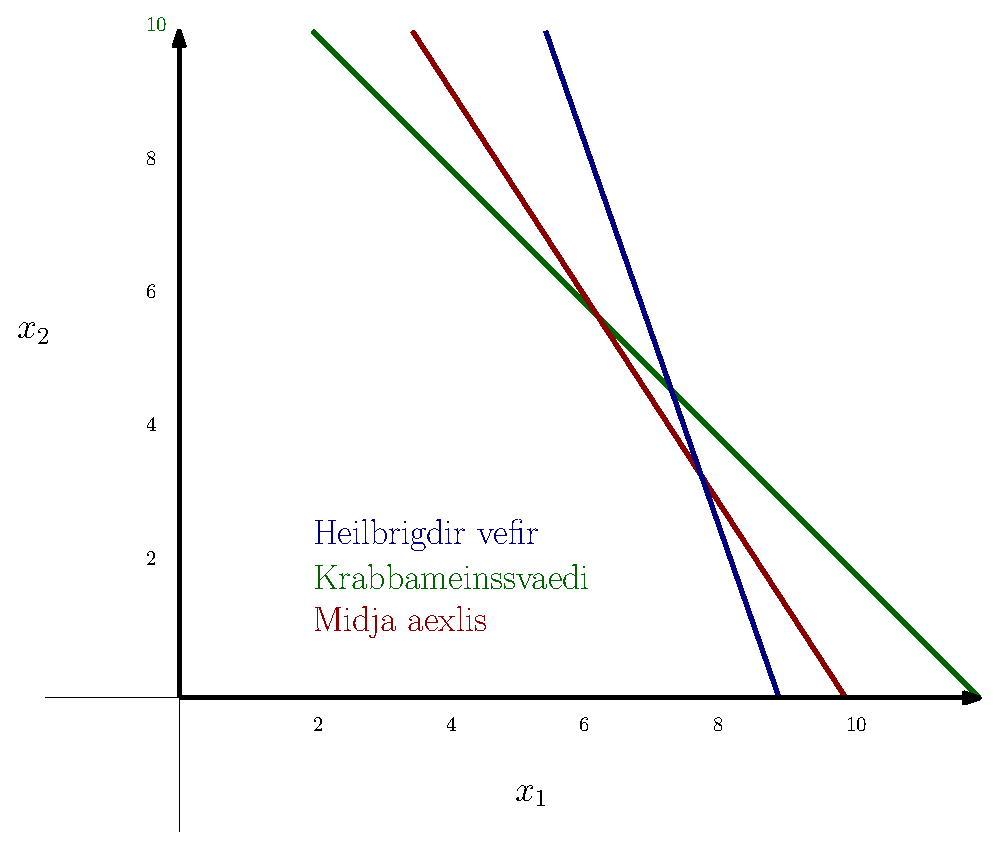
\includegraphics[width=0.8\columnwidth]{figs/cancer.eps}
\end{center}\caption{Skorður vegna geislameðferðar}  
\end{figure}

\begin{samepage}
\begin{daemi}Banki nokkur vinnur að því að marka nýja útlánastefnu. Fjórar tegundir lána verða í boði:
\begin{center}{\renewcommand{\arraystretch}{1.5} \renewcommand{\tabcolsep}{0.2cm}
\begin{tabular}{|llcc|}\hline
& Tegund & Vextir & Afskrifarhlutfall \\ \hline
1 & Lán til fyrirtækja & $r_1$ & $p_1$ \\
2 & Lán til einstaklinga (neysla/yfirdráttur) & $r_2$ & $p_2$ \\
3 & Húsnæðislán & $r_3$ & $p_3$ \\
4 & Bílalán & $r_4$ & $p_4$ \\ \hline
\end{tabular}} 
\end{center} 
Hlutfallið sem þarf að afskrifa er metið út frá fyrri reynslu, og \mbox{$0<p_i<<1$}. 
Heildarfjármagn til ráðstöfunar er $L$ (t.d. í krónum). Jafnframt hefur eftirfarandi hefur verið ákveðið á síðasta stjórnarfundi:
\begin{itemize}
 \item A.m.k. 40\% af fjármagninu fer til fyrirtækja.
 \item Húsnæðislán a.m.k. helmingur bíla og neyslulána .
 \item Hámark 5\% heildarútlána sem þarf að afskrifa.
\end{itemize}
Ákvarða þarf hagkvæmustu ráðstöfun á fjármagni bankans.
\end{daemi}
\end{samepage}
\begin{lausn}
 Ákvarðanabreytur:
 $$ x_i = \textrm{ Fjármagn sem veitt er til lánaflokks } \quad i\in\{1,2,3,4\}$$
 Markfall
 $$ \max_{\vec{x}} z = \underbrace{\sum_{i=1}^4(1-p_i)r_ix_i}_{\textrm{tekjur af lánum}} - \underbrace{\sum_{i=1}^4 p_ix_i}_{\textrm{afskriftir}} $$
 því hlutfall í skilum fyrir lánaflokk $i$ er $1-p_i$ og vaxtatekjur þess eru $r_ix_i$.

 Skorðurnar eru 
{\renewcommand{\arraystretch}{1.5} \renewcommand{\tabcolsep}{0.2cm}
\[ \begin{array}{lrcl}
  \textrm{Heildarráðstöfun:}&\sum_{i=1}^4 x_i &\leq& L \\
  \textrm{Fyrirtæki:}&x_1 &\geq& 0.4 L \\
  \textrm{Einstaklingar:}&x_3 &\geq& \frac{1}{2} \left(x_4+x_2\right) \\
  \textrm{Hámarks afskriftir:}&\sum_{i=1}^4 p_ix_i &\leq& 0.05 \sum_{i=1}^4 x_i \\
  &x_1,x_2,x_3,x_4&\geq&0
 \end{array}\]}
\end{lausn}



 

\section{Hugbúnaður fyrir línulega bestun}
\subsection{Forrit sem leysa línuleg bestunarverkefni}
Forrit sem leysa línuleg bestunarverkefni eru t.d.

\begin{tabular}{ll}
 Excel &  $\div$ skelfilegt \\
 \href{http://www.mathworks.com/products/matlab/}{Matlab} & $\div$ rándýrt, $\div$ LP föll óþæginleg í notkun fyrir stór verkefni \\
 \href{http://www-01.ibm.com/software/integration/optimization/cplex-optimizer/}{CPLEX} & + mögulega það öflugasta sem er í boði, $\div$ rándýrt \\
 \href{http://www.mosek.com/}{MOSEK} & + öflugur pakki, + sanngjarnt verð \\
 \href{http://lpsolve.sourceforge.net/5.0/}{Ip-solve} & + ókeypis \\
 \href{http://www.gnu.org/software/glpk/}{GLPK} & + ókeypis \\
 \href{http://www.gurobi.com/}{gurobi} & + ókeypis stúdenta útgáfa \\
\end{tabular}

Fyrir Windows notendur er hægt að nota forritunarumhverfið \href{http://gusek.sourceforge.net/gusek.html}{GUSEK} fyrir GLPK.
 
\subsection{Líkindamál}
Svonefnd \ath{líkanamál} (e. modelling language) eru mjög gagnleg við að skilgreina stór bestunarverkefni. Dæmi um nokkur þeirra eru t.d.

\begin{tabular}{ll}
 MPL & + þæginlegt notendaviðmót, $\div$ selt \\
 GAMS & + rótgróið, $\div$ selt \\
 AMPL & + rótgróið, $\div$ selt \\
 MATHPROG & + einföld útgáfa af AMPL, + ókeypis 
\end{tabular}

\begin{aths}Í þessu námskeiði verður stuðst við GLPK og MATHPROG\end{aths}